\section{Experimental Evaluation}
\label{sec:exp}
We are using using three different settings, $Setting = [\lambda_1, \lambda_2, \lambda_3]$, in the experiments. In $Setting_1 = [1.6, 0.35, 0.05]$, the average interaction involved three nodes (a triad), which corresponds approximately to the analyzed co-authorship network. This setting presumes the interaction is dominated by neighbors of the proactive node with the occasional participation of new nodes and rather exceptional participation of existing nodes yet not connected to the proactive node. In $Setting_2 = [3, 6, 1]$ predominate new nodes, and the average number of nodes in interaction is $11$. In $Setting_3 = [0.45, 0.45, 0.1]$ interaction involved two nodes (a dyad) on average, wherein the number of neighbors and new nodes are balanced and new connection occurrences are less likely.

\begin{figure}[ht]
	\centering
  \begin{subfigure}{2.7cm}
    \centering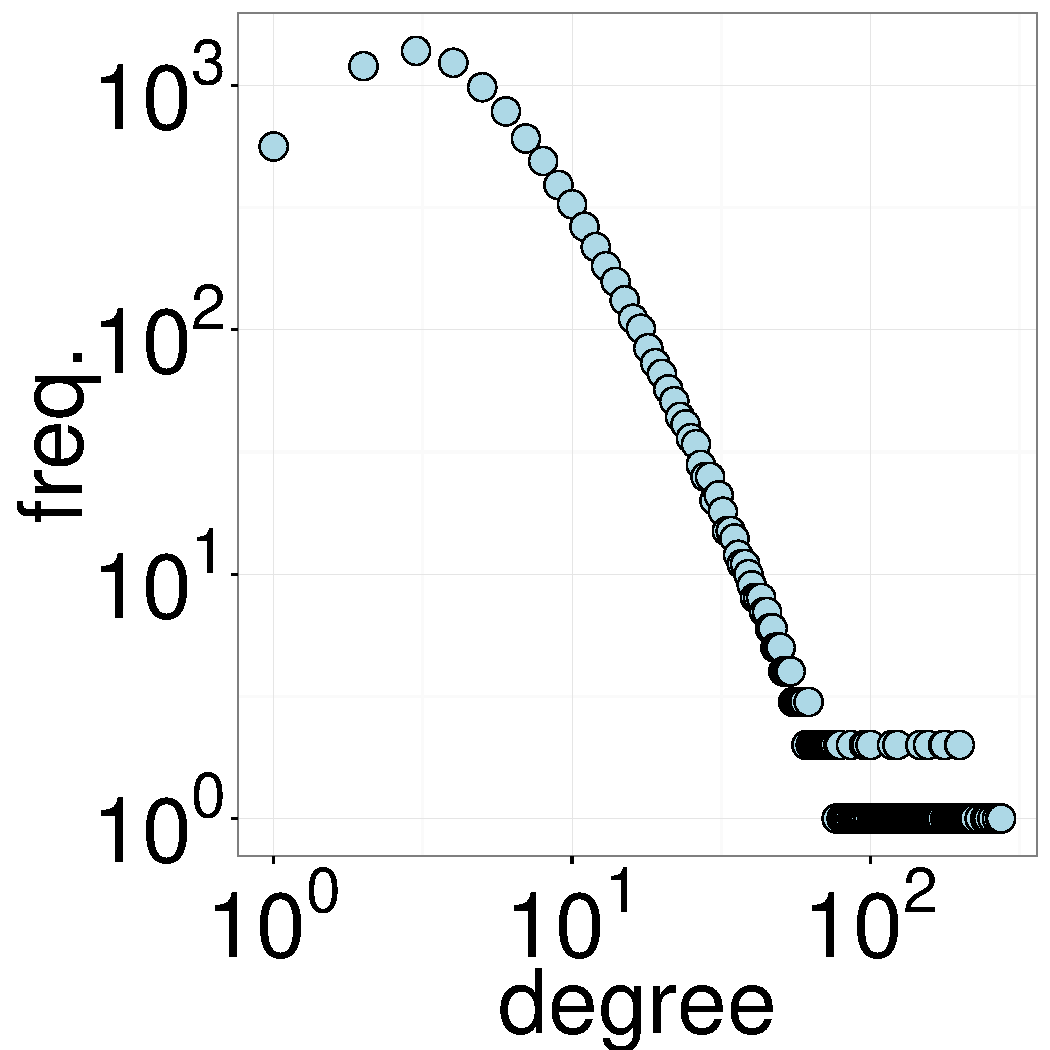
\includegraphics[width=2.5cm]{figures/distr_stupnu_Setting1}
    \caption{$Setting_1$}
  \end{subfigure}
  \begin{subfigure}{2.7cm}
    \centering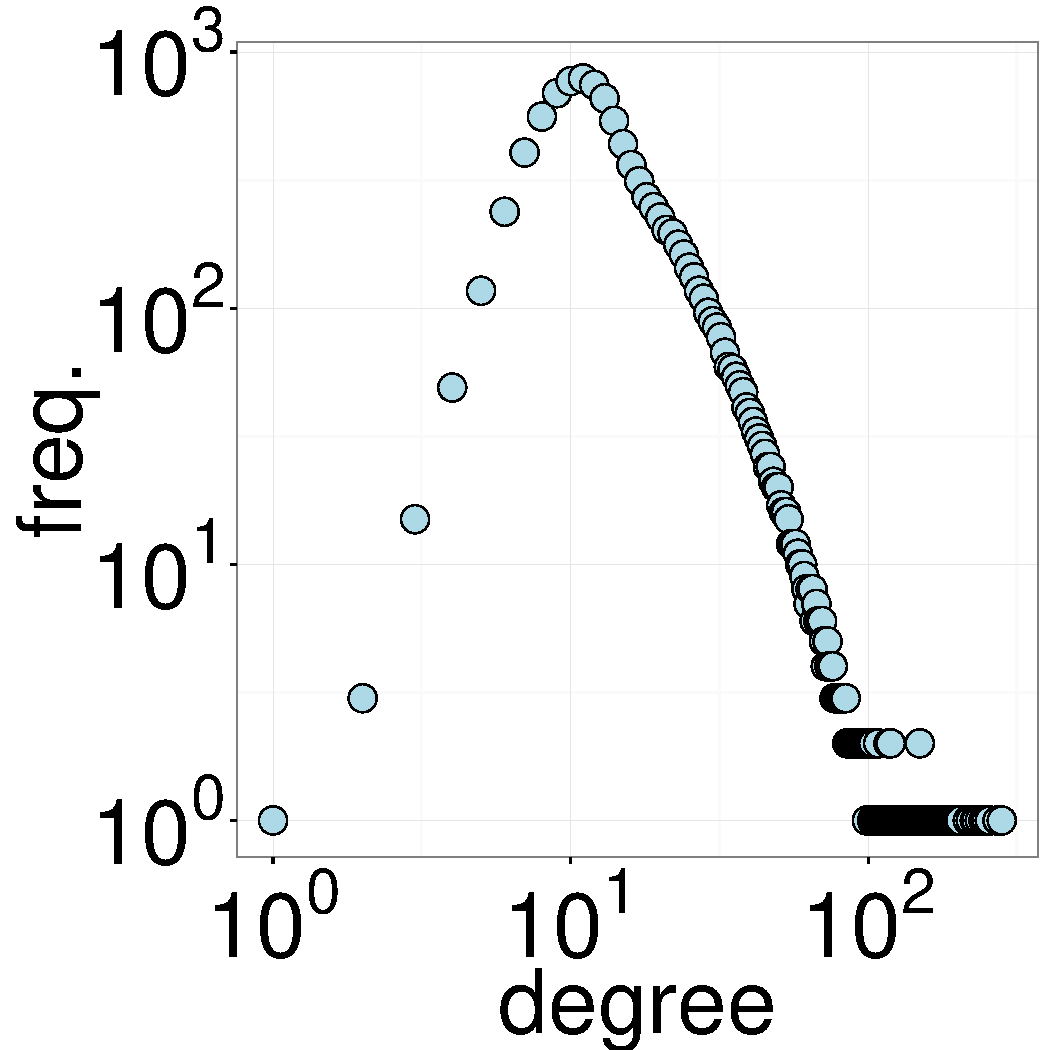
\includegraphics[width=2.5cm]{figures/distr_stupnu_Setting2}
    \caption{$Setting_2$}
		  \end{subfigure}
   \begin{subfigure}{2.7cm}
    \centering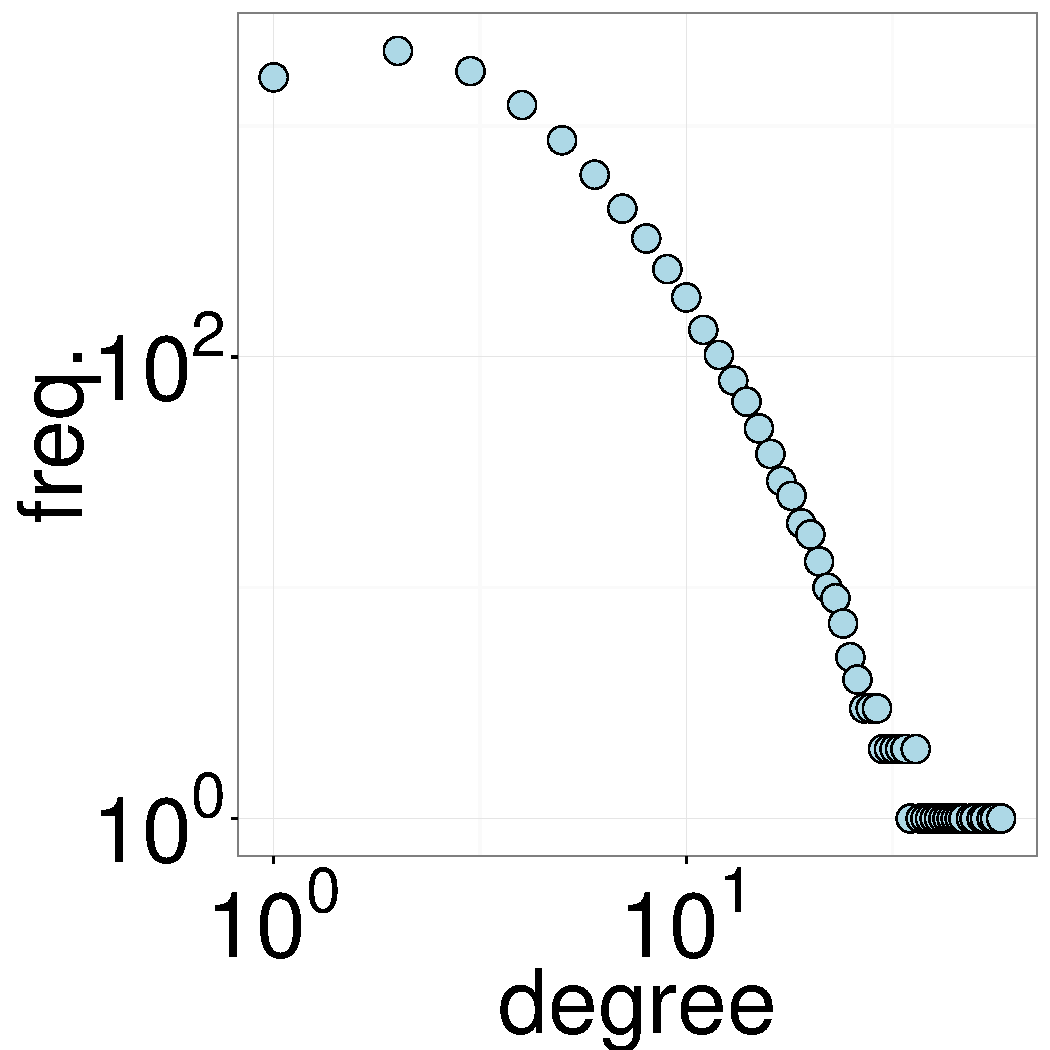
\includegraphics[width=2.5cm]{figures/distr_stupnu_Setting3}
    \caption{$Setting_3$}
  \end{subfigure}
	\caption{Degree distribution}
\label{fig:DD}
\end{figure}

\begin{figure}[ht]
	\centering
  \begin{subfigure}{2.7cm}
    \centering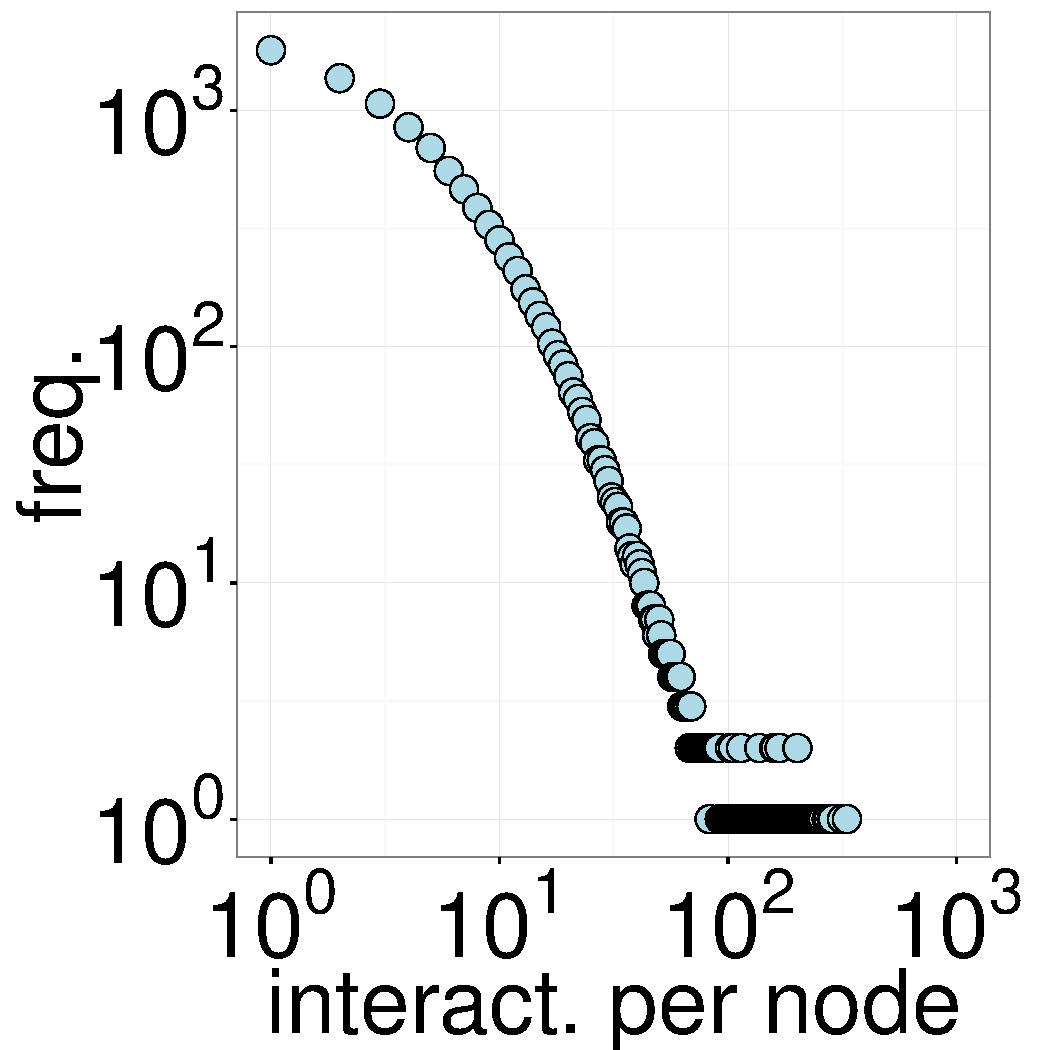
\includegraphics[width=2.5cm]{figures/inter_per_vert_Setting1}
    \caption{$Setting_1$}
  \end{subfigure}
  \begin{subfigure}{2.7cm}
    \centering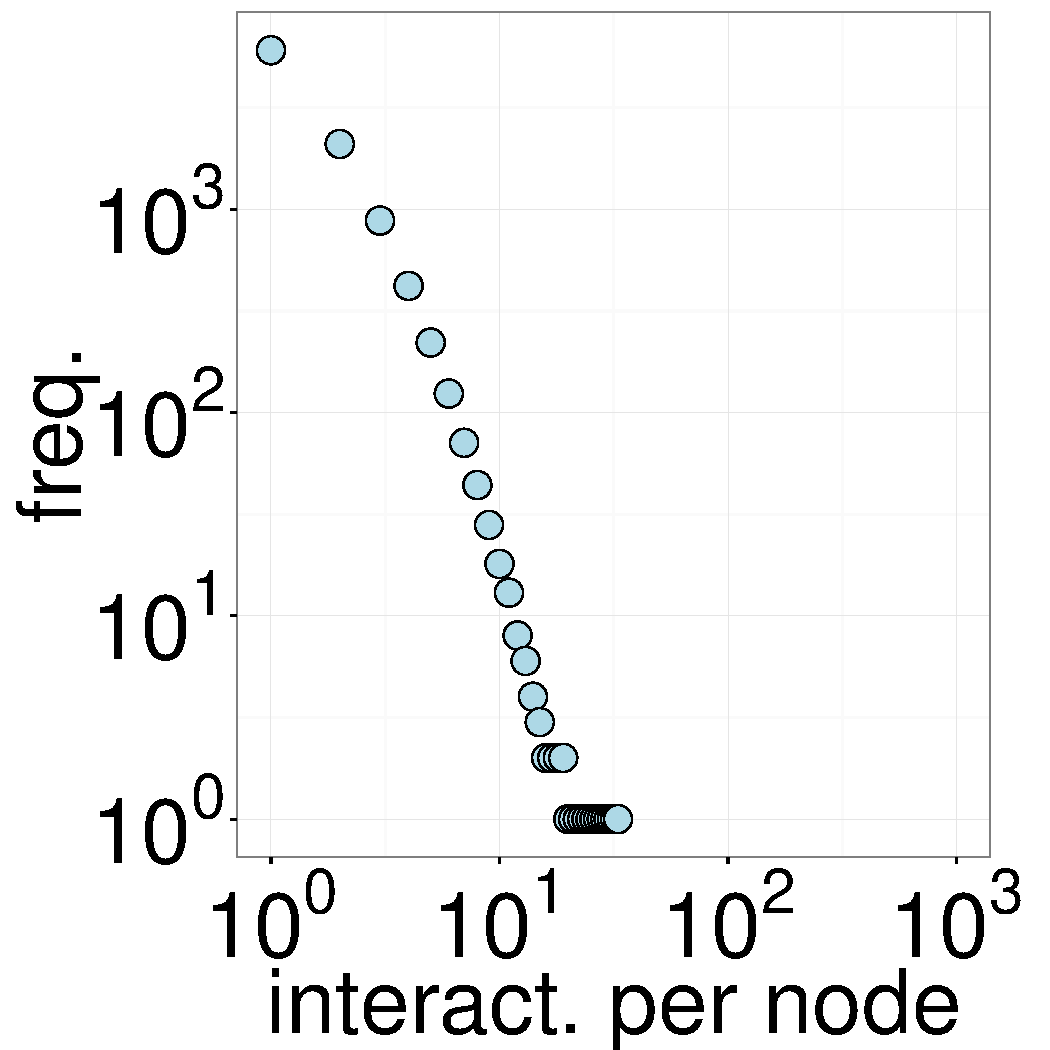
\includegraphics[width=2.5cm]{figures/inter_per_vert_Setting2}
    \caption{$Setting_2$}
		  \end{subfigure}
   \begin{subfigure}{2.7cm}
    \centering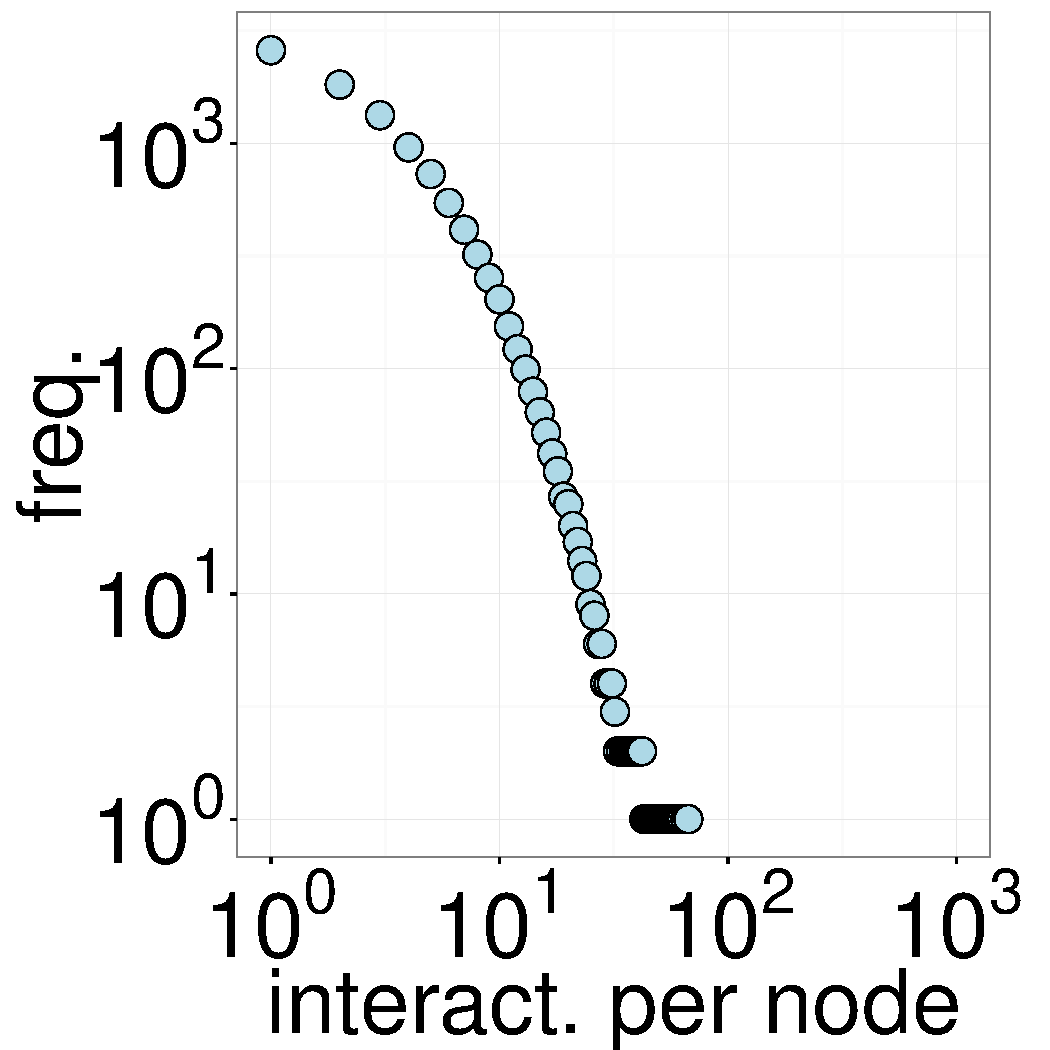
\includegraphics[width=2.5cm]{figures/inter_per_vert_Setting3}
    \caption{$Setting_3$}
  \end{subfigure}
	\caption{Interactions per	node}
\label{fig:IpN}
\end{figure}

\begin{figure}[ht]
	\centering
  \begin{subfigure}{2.7cm}
    \centering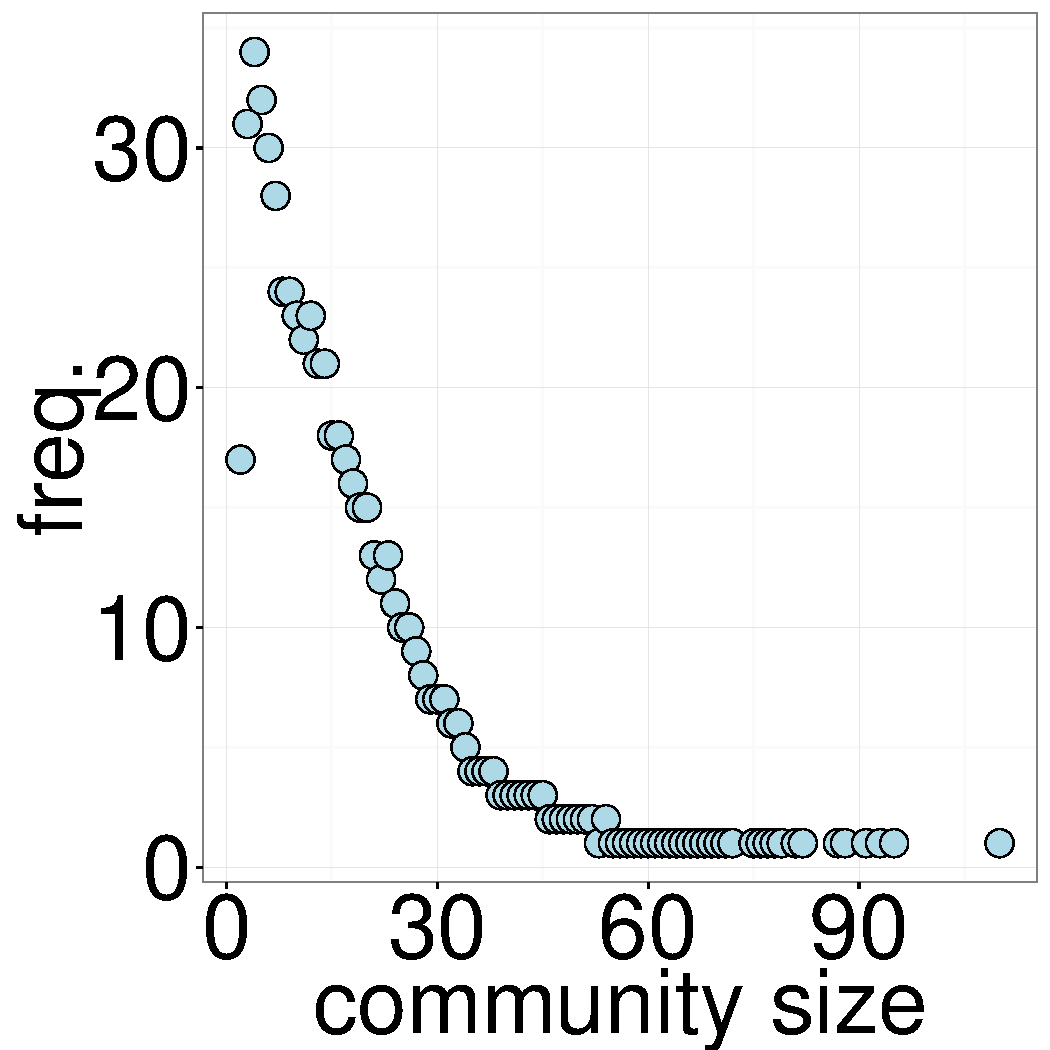
\includegraphics[width=2.5cm]{figures/dist_vel_komf_Setting1}
    \caption{$Setting_1$}
  \end{subfigure}
  \begin{subfigure}{2.7cm}
    \centering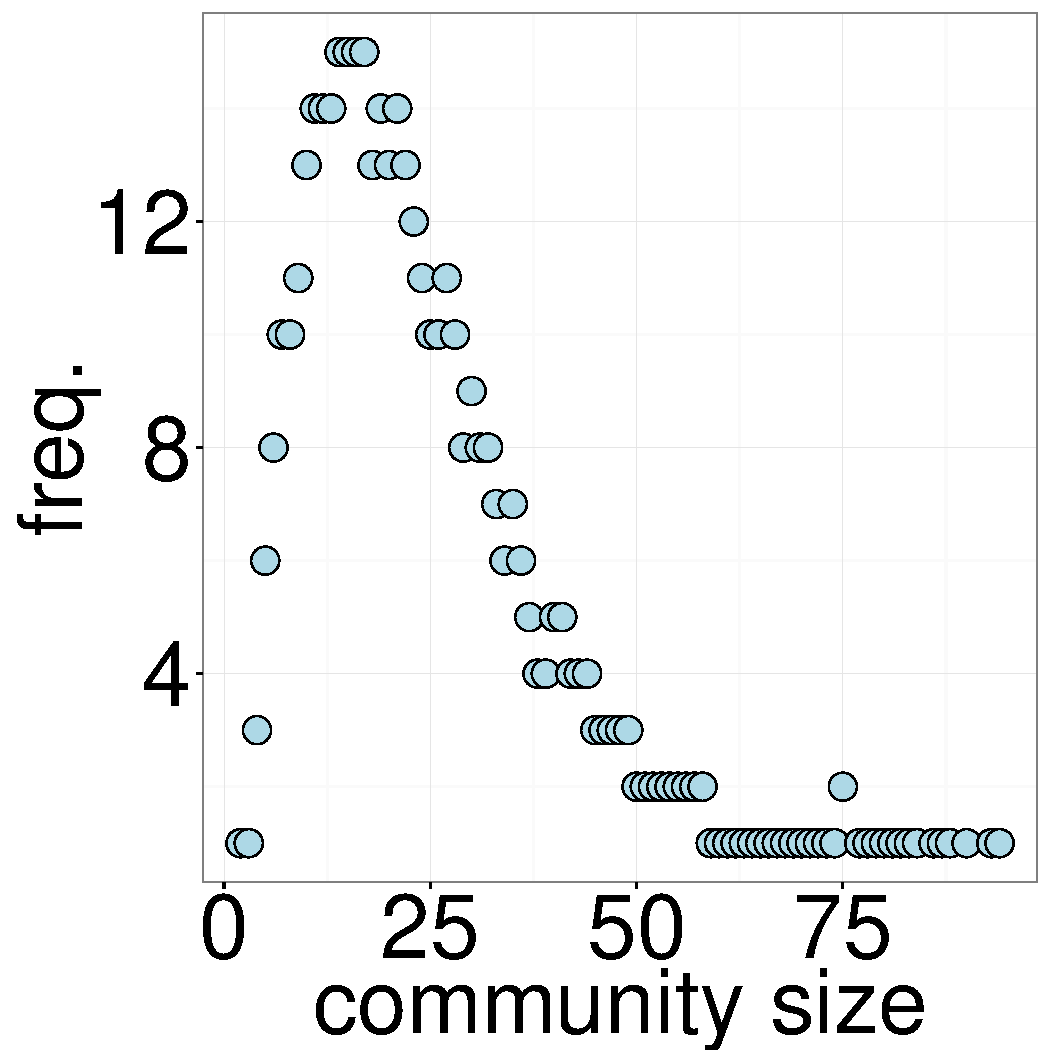
\includegraphics[width=2.5cm]{figures/dist_vel_komf_Setting2}
    \caption{$Setting_2$}
		  \end{subfigure}
   \begin{subfigure}{2.7cm}
    \centering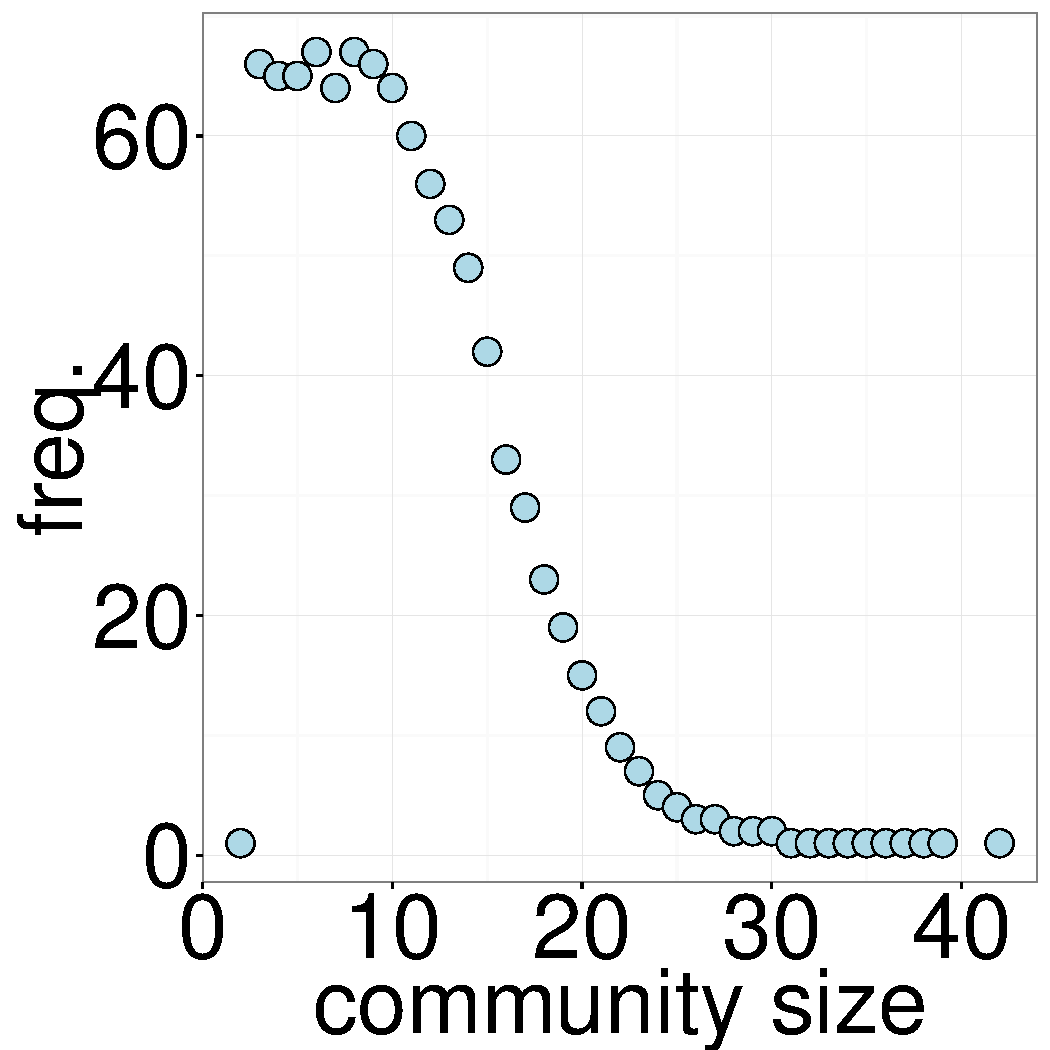
\includegraphics[width=2.5cm]{figures/dist_vel_komf_Setting3}
    \caption{$Setting_3$}
  \end{subfigure}
	\caption{Community size}
\label{fig:ComSize}
\end{figure}


\subsection{Properties of Generated Network}

\begin{table*}[ht]
  \centering
  \caption{Global properties}
		\begin{tabular}{|c|r|rrrrrrrrrrr|}
\hline
Setting &  & $n$ & $m$ & $<$k$>$ &  $<$l$>$ & $l_{max}$ & $CC$ & $r$ & $com_{IM}$ & $com_L$ & $Q_{IM}$ & $Q_L$ \\ 
\hline
$Setting_1$ & mean & 10001.10 & 40108.97 & 8.0209 & 4.8101 & 12.07 & 0.6555 & 0.14522 & 609.40 & 54.70 & 0.6424 & 0.7119 \\ 
& sd & 0.31 & 398.80 & 0.0797 & 0.0421 & 0.64 & 0.0029 & 0.01769 & 12.37 & 7.04 & 0.0062 & 0.0085 \\ 
\hline	
$Setting_2$ & mean & 10003.87 & 88620.40 & 17.7172 & 4.2369 & 8.43  & 0.8087 & 0.12961 & 422.60 & 42.90 & 0.6772 & 0.7334 \\ 
& sd & 1.53 & 797.95 & 0.1600 & 0.0277 & 0.63  & 0.0018 & 0.00913 & 10.30 & 2.78 & 0.0049 & 0.0067 \\ 
\hline
$Setting_3$ & mean & 10001.17 & 21494.57 & 4.2984 & 6.8965 & 16.23 & 0.4784 & 0.19907 & 953.30 & 68.70 & 0.7276 & 0.8129 \\ 
&  sd & 0.46 & 142.64 & 0.0285 & 0.0609 & 0.63 & 0.0044 & 0.01222 & 15.55 & 3.19 & 0.0035 & 0.0038 \\ 
\hline
\end{tabular}%
  \label{tab:gp}%
\end{table*}%
\begin{table}[ht]
  \centering
  \caption{Interactions}
\begin{tabular}{|r|r|rrr|}
	\hline
Setting & & $I$ & $<$i$>$ & $<$s$>$ \\ 
\hline
$Setting_1$ & mean & 28561.90 & 8.0887 & 2.8323 \\ 
&  sd & 278.93 & 0.0817 & 0.0082 \\ 
\hline	
$Setting_2$ & mean & 1664.53 & 1.8278 & 10.9860 \\ 
& sd & 17.69 & 0.0115 & 0.0824 \\
\hline	
$Setting_3$ & mean & 22204.43 & 4.3772 & 1.9716 \\ 
& sd & 202.06 & 0.0292 & 0.0069 \\ 
\hline
	\end{tabular}%
  \label{tab:interact}%
\end{table}%

In the first experiment, we show the properties of networks generated with different settings. We generated for each setting $100$ networks with approximately $10000$ nodes. Table \ref{tab:gp} summarizes average values (and standard deviation) of measured properties for each setting. Measured properties include number of nodes $n$ and edges $m$, average degree $<$k$>$, average shortest path length $<$l$>$, diameter $L_{max}$, average clustering coefficient $CC$, assortativity $r$, number of communities detected by Infomap \cite{rosvall2009map} $com_{IM}$ and Louvain \cite{blondel2008fast} $com_L$ algorithm, and corresponding modularities $Q_{IM}$ and $Q_L$, respectively. Table \ref{tab:interact} contains average values associated with the temporality of the network, i.e. total number of interactions $I$, average number of interactions $<$i$>$ and average number of nodes in interaction $<$s$>$. Figures \ref{fig:DD}-\ref{fig:ComSize} show degree distribution, number of interactions distribution and distributions of community size detected by Infomap algorithm.

The experiment indicates that all three settings generate networks with small-world and scale-free characteristics. The first and second setting have generated networks of high average clustering coefficient. Networks have a tendency to be assortative. Assortativity values correspond to all settings to the values known from social networks \cite{newman2002assortative}. Generated networks also have community structure and a high modularity for all settings.

\begin{figure}[ht]
\centering
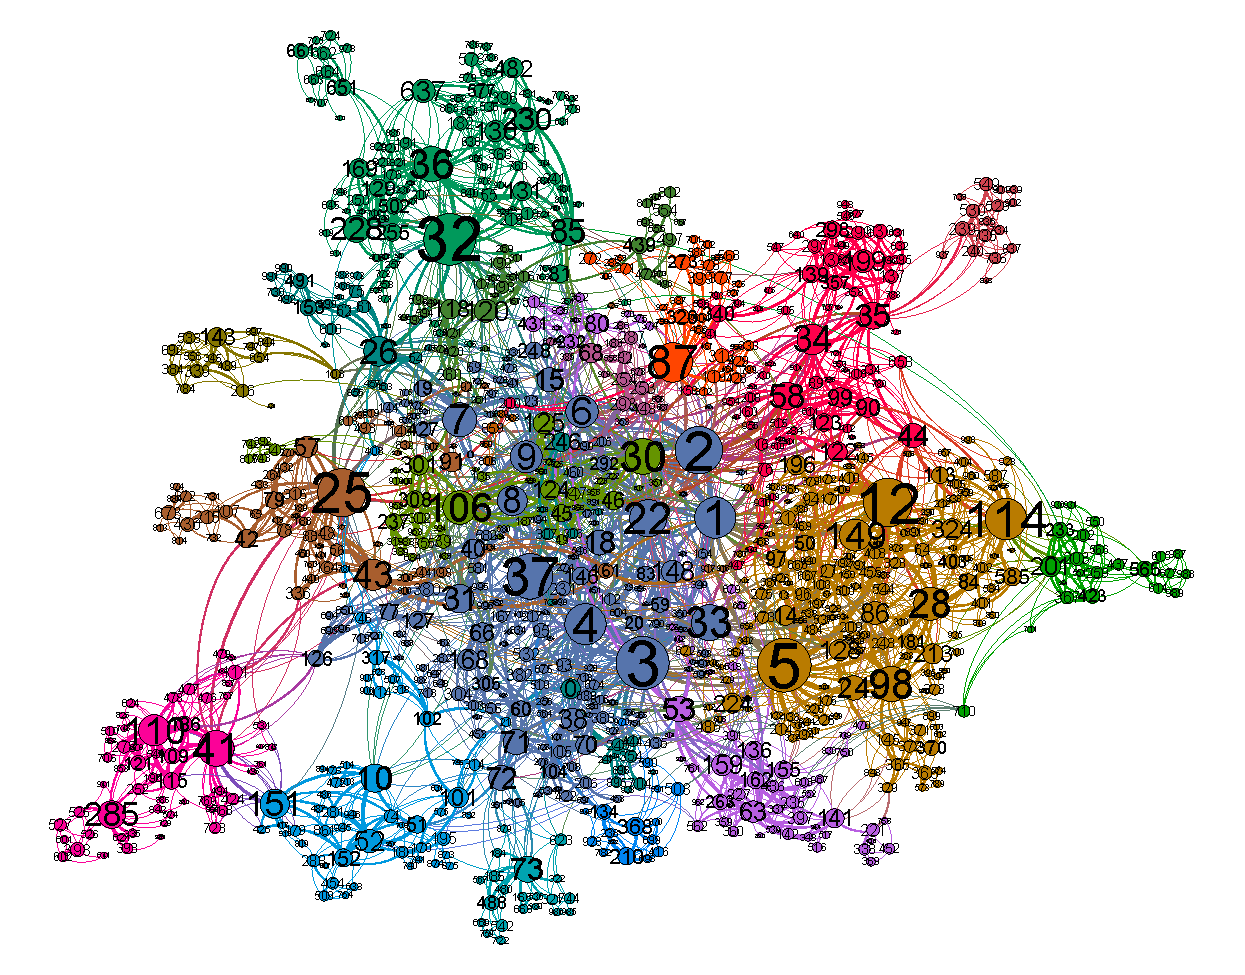
\includegraphics[width=\linewidth]{figures/setting1_1000}
  \caption{Network: 1000 nodes, $Setting_1$}
	\label{fig:Set1000}
\end{figure}

Figure \ref{fig:Set1000} shows a network with $1000$ nodes and $3599$ edges generated with $Setting_1$. A total of $2830$ interactions took place. The size of nodes and strength of edges correspond to the number of interactions they took part in, the labels indicate the order in which nodes were created. The network has an overlapping community and core-periphery structure. Colored 19 communities were detected by Louvain method, modularity is $0.746$.

\subsection{Evolution of Generated Network}
The subject of the second experiment is one network generated with $Setting_1$. The aim is to show the development of network properties during its growth. The values for each characteristic are measured when the network has $10, 20, 50, 100$, ..., and $10000$ nodes. The results are summarized in Table \ref{tab:Evolut}.

\begin{table*}[ht]
  \centering
  \caption{Evolution of network properties}
	\begin{tabular}{|r|rrrrrrrrrr|}

\hline
  $n$ & $m$ & $<$k$>$ &  $<$l$>$ & $l_{max}$ & $CC$ & $r$ & $com_{IM}$ & $com_L$ & $Q_{IM}$ & $Q_L$ \\
\hline
  10 & 27.00 & 5.4000 & 1.4000 & 20 & 0.8195 & -0.41738 & 1 & 3 & 0.0000 & 0.0590 \\ 
 20 & 53.00 & 5.3000 & 2.0684 & 5 & 0.5804 & -0.09355 & 2 & 4 & 0.0361 & 0.2398 \\ 
  50 & 184.00 & 7.3600 & 2.5004 & 7 & 0.6248 & -0.00886 & 5 & 5 & 0.2957 & 0.3742 \\ 
100 & 388.00 & 7.7600 & 2.8731 & 6 & 0.6793 & 0.09177 & 11 & 9 & 0.4259 & 0.4613 \\ 
 200 & 812.00 & 8.1200 & 3.1859 & 7 & 0.6824 & 0.05107 & 20 & 11 & 0.5002 & 0.5121 \\ 
500 & 2112.00 & 8.4480 & 3.6095 & 8 & 0.6394 & 0.11911 & 44 & 11 & 0.5540 & 0.5849 \\ 
 1000 & 4053.00 & 8.1060 & 3.9402 & 9 & 0.6592 & 0.14528 & 83 & 17 & 0.5812 & 0.6341 \\ 
2000 & 8306.00 & 8.3060 & 4.2054 & 10 & 0.6538 & 0.14016 & 151 & 24 & 0.5972 & 0.6714 \\ 
5000 & 20316.00 & 8.1264 & 4.5344 & 12 & 0.6603 & 0.15823 & 342 & 44 & 0.6203 & 0.6827 \\ 
10000 & 40476.00 & 8.0952 & 4.8015 & 11 & 0.6557 & 0.15351 & 645 & 64 & 0.6307 & 0.7003 \\ 
\hline
  \end{tabular}
	  \label{tab:Evolut}%
\end{table*}%
	
Figure \ref{fig:EvolNet}, similarly to the previous experiment, shows the distribution of degree, number of interactions and size of communities. The evolution of these properties is portrayed when network has $100, 200, 1000, 5000, 10000$ nodes.

\begin{figure*}[ht]
\centering
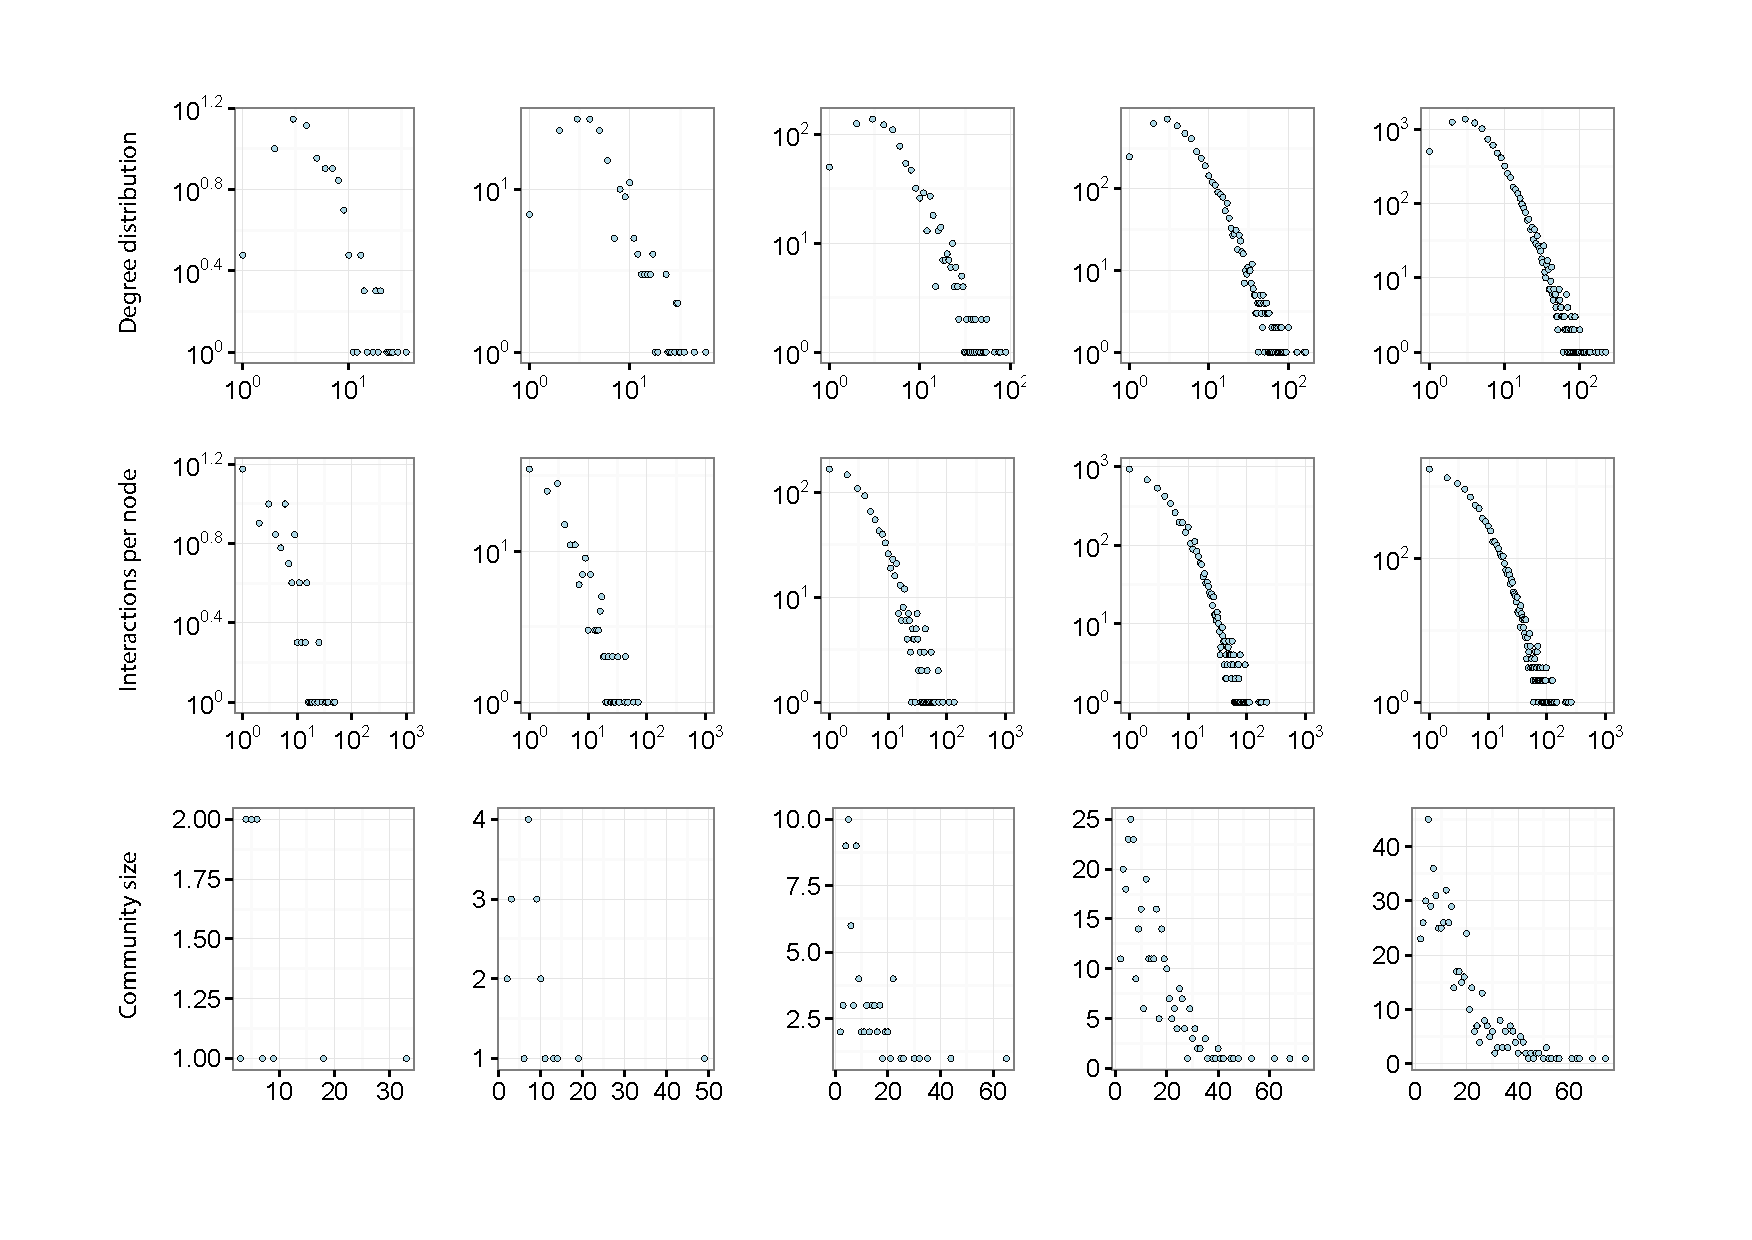
\includegraphics[width=46em]{figures/distribution_10_20_50}
\caption{Evolution of network (100, 200, 1000, 5000, 10000 nodes)}
\label{fig:EvolNet}
\end{figure*}

Key properties (average degree, shortest path, clustering coefficient, assortativity, modularity) happen to stabilize their values between $1000$ and $10000$ nodes. Our experiments show that  generated networks with other settings also have similar behavior. Figure \ref{fig:InterEvol} shows the evolution of the number of interactions for fifteen nodes with the highest number of interactions at the end of the generation process. The ID of a node represents the moment of its creation. The trend shows how the chances of participating in interactions increase for nodes that already have a high number of interactions.

\begin{figure}[ht]
\centering
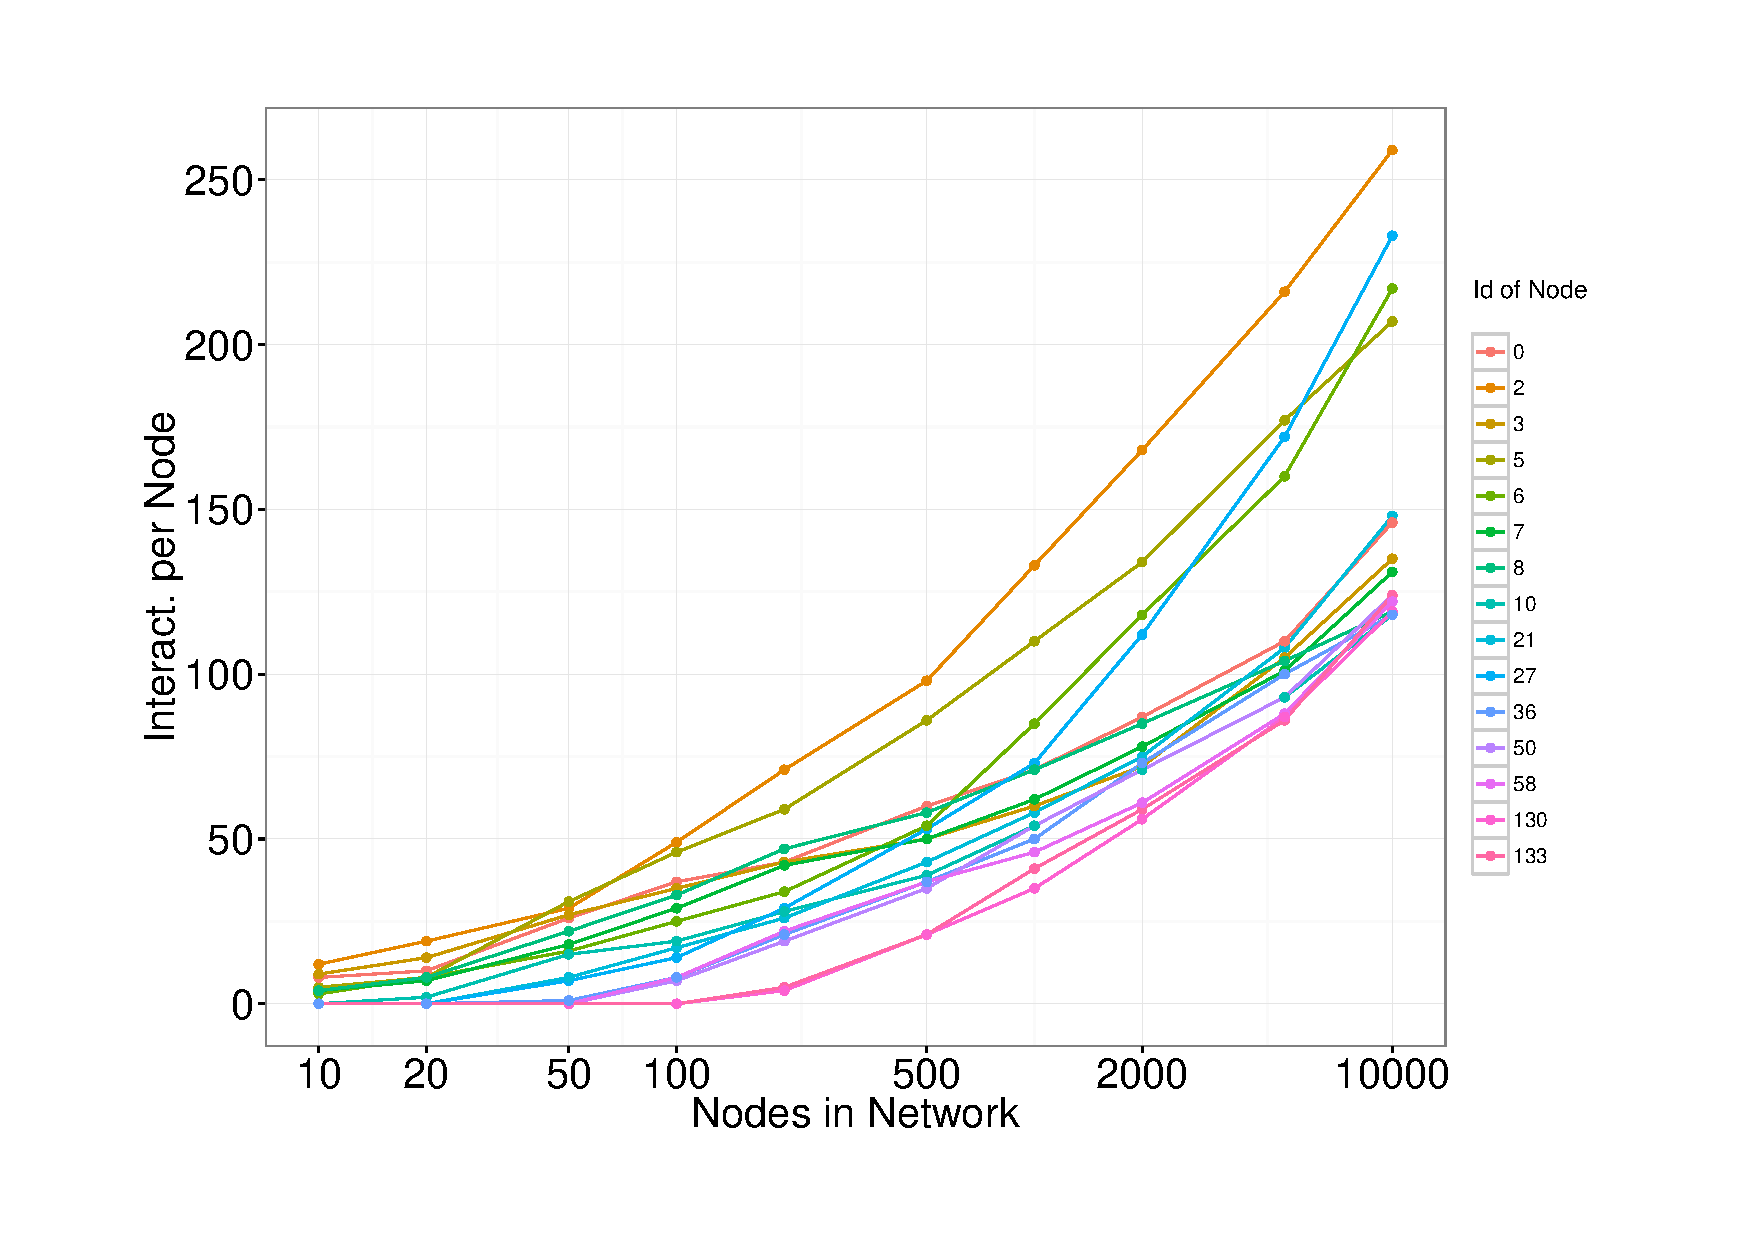
\includegraphics[width =\linewidth]{figures/Interaction_evolution}
\caption{Evolution of nodes with the most interactions}
\label{fig:InterEvol}
\end{figure}


\subsection{Correlations}
In this experiment, we compare the analyzed real-world network with generated networks. For each setting we generated a network with one million nodes. Then we examined the correlation between the node's creation time and it's degree and number of interactions, respectively. The emergence of the node is represented by its $ID$, which is in the order of its creation. Furthermore, we calculated the correlation between degree and number of node's interactions. We did the same for the analyzed DBLP dataset, where the order of nodes is to be understood as an estimate based on data pre-processing described in Section \ref{sec:dblp}.

\begin{table}[ht]
  \centering
  \caption{Correlations}
\begin{tabular}{|r|rrr|}
	\hline
Setting & $\rho(Id, k)$ & $\rho(Id, i)$ & $\rho(k, i)$ \\ 
\hline
$Setting_1$ & -0.59 & -0.50 & 0.96 \\  
\hline	
$Setting_2$ & -0.47 & -0.47 & 0.95 \\ 
\hline	
$Setting_3$ & -0.70 & -0.58 & 0.87 \\ 
\hline
DBLP & -0.23 & -0.18 & 0.84 \\ 
\hline
	\end{tabular}%
  \label{tab:corr}%
\end{table}%

The results summarized in Table \ref{tab:corr} show that regardless of the setting, the first two correlations are much higher in the 3-lambda model than in the DBLP dataset (Pearson's correlation coefficient was used). Thus, in the presented model, older nodes have a higher (and continuous) chance to participate in interactions than in reality. The cause is probably the aging of nodes in real-world networks where nodes, at different times, no longer participate in interactions. This significantly affects the evolution (growth) and some properties of the network.

Previous experiments demonstrated that despite the absence of aging, generated networks have very good properties. We have not, therefore, for reasons of simplicity, incorporated any of the known models of aging (e.g. inspired by \cite{dorogovtsev2000evolution, xu2010evolutionary}) to the 3-lambda network model.